% -*- TeX-master: "oving04"; -*-
\oppgaver{5}



\begin{oppgave}
Sjekk om vektorene 
	$$
	\begin{bmatrix}
	8  \\
	-8 \\
	-4 \\
	-6
	\end{bmatrix},
	\begin{bmatrix}
	-7  \\
	-7 \\
	5 \\
	6
	\end{bmatrix},
	\begin{bmatrix}
	0  \\
	3 \\
	-8 \\
	-4
	\end{bmatrix}
	$$ er lineært uavhengige.
\end{oppgave}

\begin{losning}
De er lineært uavhengige.
\end{losning}





\begin{oppgave}

\begin{punkt}
Sjekk at vektorene $$\begin{bmatrix}
1\\
5\\
-3
\end{bmatrix}, \quad \begin{bmatrix}
4\\
18\\
4
\end{bmatrix}$$ er lineært uavhengige.
\end{punkt}

\begin{punkt}
Finn en tredje vektor $\V{v}$ som sammen med vektorene i $\textbf{a)}$ er lineært uavhengige.
\end{punkt}


\begin{punkt}
Vis at $\V{v}$ og vektorene i $\textbf{a)}$ til sammen spenner ut $\mathbb{R}^3$. Sammenlign med oppgave \textbf{9.} \textbf{b)} kapittel 3.
\end{punkt}

\end{oppgave}

\begin{losning}

\begin{punkt}
Radreduser matrisen med oppgitte vektorer som kolonner eller sjekk at ikke $$\begin{bmatrix}
1\\
5\\
-3
\end{bmatrix}=c\begin{bmatrix}
4\\
18\\
4
\end{bmatrix}$$ for et tall $c$ direkte.
\end{punkt}

\begin{punkt}
Lik fremgangsmåte som oppgave 5 kapittel 3.

\noindent
Merk: Å finne en vektor som er lineært uavhengig av vektorene i \textbf{a)} svarer altså til å finne en vektor som ikke er en lineærkombinasjon av vektorene i \textbf{a)}. 
\end{punkt}

\begin{punkt}
Teorem \ref{thm:linuavhspan} gir at de tre vektorene spenner ut $\mathbb{R}^3$.

Vektoren du fant i \textbf{b)} løser oppgave \textbf{9.} \textbf{b)} kapittel 3; husk at informasjonen om et andregradspolynom $p(x)=ax^2+bx+c$ kan lagres -- entydig -- i en vektor $$\V{p}=\begin{bmatrix}
a\\
b\\
c
\end{bmatrix}.$$ De
\end{punkt}

\end{losning}






\begin{oppgave}
\begin{punkt}
Sjekk om vektorene $$
\begin{bmatrix}
1\\
2\\
3
\end{bmatrix}, \quad \begin{bmatrix}
2\\
3\\
4
\end{bmatrix}, \quad \begin{bmatrix}
3\\
4\\
5
\end{bmatrix}
$$
er lineært uavhengige.
\end{punkt}

\begin{punkt}
Finn en vektor $\V{v}$ som er lineært uavhengig av alle vektorene i $\textbf{a)}$.
\end{punkt}

\begin{punkt}
Bruk teorien om lineært uavhengige vektorer til å vise at vektorene i $\textbf{a)}$ og vektoren $\V{v}$ til sammen spenner ut $\mathbb{R}^3$.
\end{punkt}
\end{oppgave}

\begin{losning}

\begin{punkt}
Ved å radredusere matrisen $$A=\begin{bmatrix}
1 & 2 & 3\\
2 & 3 & 4\\
3 & 4 & 5
\end{bmatrix}$$ ser vi at vi får en fri variabel dersom vi prøver å løse $A\V{x}=\V{0}$. Eller ekvivalent har vi ikke et lederelement i hver rad. Teorem \ref{thm:linuavh} sier da at vektorene er lineært avhengige.
\end{punkt}

\begin{punkt}
Lik fremgangsmåte som i del $\textbf{b)}$ av forrige oppgave.
\end{punkt}


\begin{punkt}
Du kan sjekke at to vilkårlige vektorer fra $\textbf{a)}$ og vektoren du fant i $\textbf{b)}$ er lineært uavhengige. Det er altså tre lineært uavhengige vektorer i det lineære spanet til vektorene i \textbf{a)} og \textbf{b)}. Derfor spenner vektorene $\mathbb{R}^3$ (Teorem \ref{thm:linuavhspan}).
\end{punkt}

\end{losning}









\begin{oppgave}
Finn ut om følgende påstander er sanne eller ikke.
\begin{punkt}
Hvis tre vektorer $\V{u}$, $\V{v}$ og~$\V{w}$ er lineært
avhengige, så finnes det to tall $a$ og~$b$ slik at: 
\[
\V{u} = a \cdot \V{v} + b \cdot \V{w}
\]
\end{punkt}

\begin{punkt}
Vi må ha $n$ lineært uavhengige vektorer for å spenne ut $\mathbb{R}^n$
\end{punkt}

\begin{punkt}
La $m>n$. Vi kan ha $m$ lineært uavhengige vektorer i $\mathbb{R}^n$.
\end{punkt}

\end{oppgave}

\begin{losning}
Påstand \textbf{a)} og \textbf{b)} er sanne; \textbf{c)} er ikke.
\end{losning}








\begin{oppgave}
De to bildene viser vektorer i $\mathbb{R} ^2$. 
	
\begin{punkt}
Er vektorene $\V{v}_1$ og~$\V{v}_2$ lineært uavhengige? Utspenner de $\mathbb{R} ^2$? Begrunn svarene dine.
\begin{center}
	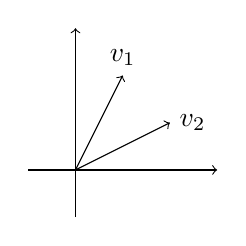
\begin{tikzpicture}[scale=0.6]
	\draw[->,above] (0,0) node{} -- (1,2) node{$\V{v}_1$};
	\draw[->, right] (0,0) node{} -- (2,1) node{$\V{v}_2$};
	\draw[->] (-1,0) {} -- (3,0) {};
	\draw[->] (0,-1) {} -- (0,3) {};
	\end{tikzpicture}
\end{center}
\end{punkt}



\begin{punkt}
Er vektorene $\V{v}_1$, $\V{v}_2$ og~$\V{v}_3$ lineært uavhengige? Utspenner de $\mathbb{R} ^2$? Begrunn svarene dine.
\begin{center}
	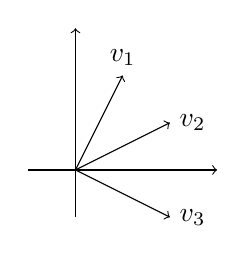
\begin{tikzpicture}[scale=0.6]
	\draw[->,above] (0,0) node{} -- (1,2) node{$\V{v}_1$};
	\draw[->, right] (0,0) node{} -- (2,1) node{$\V{v}_2$};
	\draw[->, right] (0,0) node{} -- (2,-1) node{$\V{v}_3$};
	\draw[->] (-1,0) {} -- (3,0) {};
	\draw[->] (0,-1) {} -- (0,3) {};
	\end{tikzpicture}
\end{center}
\end{punkt}
\end{oppgave}

\begin{losning}

\begin{punkt}
Ja, de er lineært uavhengige. Ja, de spenner ut $\mathbb{R}^2$.
\end{punkt}

\begin{punkt}
Nei, de er ikke lineært uavhengige. Ja, de spenner ut $\mathbb{R}^2$.
\end{punkt}

\end{losning}


\begin{oppgave}
\begin{punkt}
Betrakt vektorene
\[ 
\begin{bmatrix} \;1\; \\ \;2\; \end{bmatrix}, 
\begin{bmatrix} \;2\; \\ \;3\; \end{bmatrix}, \dots, 
\begin{bmatrix} \;99\; \\ \;100\; \end{bmatrix}
\]
i $\mathbb{R}^2$. Vis at de utspenner $\mathbb{R}^2$. Er de lineært uavhengig? Begrunn svaret ditt.
\end{punkt}

\begin{punkt}
Betrakt vektorene
\[ 
\begin{bmatrix} 
\;1\; \\ 
\;\vdots\; \\ 
\;99\; 
\end{bmatrix}
\text{ og }
\begin{bmatrix} 
\;2\; \\ 
\;\vdots\; \\ 
\;100\; 
\end{bmatrix}
\]
i $\mathbb{R}^{99}$. Er de lineært uavhengige? Spenner de ut $\mathbb{R}^{99}$? Begrunn svarene dine.

\end{punkt}
\end{oppgave}

\begin{losning}

\begin{punkt}
Ja, de er lineært uavhengige. Dette kan sjekkes direkte ved å utforske om likningen 
\[ 
\begin{bmatrix} 
\;1\; \\ 
\;\vdots\; \\ 
\;99\; 
\end{bmatrix}
=c
\begin{bmatrix} 
\;2\; \\ 
\;\vdots\; \\ 
\;100\; 
\end{bmatrix}
\] har noen løsning for tallet $c$. Nei, de spenner ikke ut $\mathbb{R}^{99}$; en trenger minst nittini vektorer for å få til dette (Teorem \ref{thm:linuavhspan}).
\end{punkt}

\begin{punkt}
Nei, de er ikke lineært uavhengige; en kan maksimalt ha to lineært uavhengige vektorer i $\mathbb{R}^2$ (Teorem \ref{thm:linavhspan}). Ja, de spenner ut $\mathbb{R}^2$; samlingen inneholder to lineært uavhengeige vektorer (Teorem \ref{thm:linuavhspan}).
\end{punkt}

\end{losning}


\begin{oppgave}
La $A$ være en $m \times n$-matrise, og la $\V{v}_1$, $\V{v}_2$,
\ldots, $\V{v}_t$ være vektorer i~$\R^n$.  Finn ut om følgende
påstander er sanne eller ikke (gi et bevis eller et moteksempel).
\begin{punkt}
Hvis $\V{v}_1$, $\V{v}_2$, \ldots, $\V{v}_t$ er lineært uavhengige, så
er $A \V{v}_1$, $A \V{v}_2$, \ldots, $A \V{v}_t$ også lineært
uavhengige.
\end{punkt}
\begin{punkt}
Hvis $A \V{v}_1$, $A \V{v}_2$, \ldots, $A \V{v}_t$ er lineært
uavhengige, så er $\V{v}_1$, $\V{v}_2$, \ldots, $\V{v}_t$ også lineært
uavhengige.
\end{punkt}
\end{oppgave}

\begin{losning}

\begin{punkt}
Feil.

\noindent
Hint: Husk at matriseproduktet $A\V{v}$ er en lineærkombinasjon av kolonnene til $A$ med komponentene til $\V{v}$ som koeffisienter. Det finnes mange moteksempler \ldots 

Mer Hint: Det kan være lurt å velge $A$ slik at kolonnene er lineært avhengige.
\end{punkt}


\begin{punkt}
Riktig.

\noindent
Spesialtilfellet $t=2$: Antagelsen er at $A\V{v}_1$ og $A\V{v}_2$ er lineært uavhengige. 

Den kritiske observasjonen for å løse oppgaven: regneregler for matriser gir oss at hvis $\V{u}=c\V{w}$, så $$A\V{u}=A(c\V{w})=c(A\V{w}).$$ To vektorer som ligger på samme linje -- er lineært avhengige -- ligger altså fortsatt på samme linje etter multiplikasjon med $A$ (rent geometrisk).

Logisk konklusjon: Men vektorene $A\V{v}_1$ og $A\V{v}_2$ er antatt lineært uavhengig, de ligger altså ikke på samme linje. Derfor kan ikke $\V{v}_1$ og $\V{v}_2$ være lineært avhengig; hvis de var lineært avhengig ville $A\V{v}_1$ og $A\V{v}_2$ vært lineært avhengig basert på observasjonen ovenfor.

Kan du nå løse oppgaven for en generell $t>1$? 

\noindent
Hint: 'ligger på linje' betyr lineært avhengig i løsningen ovenfor.

\end{punkt}



\end{losning}



\begin{oppgave}
Vis at påstand 1. og 2. i teorem \ref{thm:linuavh} er ekvivalente.
\end{oppgave}

\begin{losning}
Hint: likningen $A\V{x}=\V{0}$ er ekvivalent med at en lineærkombinasjon av kolonnene til $A$ er lik null-vektoren. Hva er definisjonen på lineær uavhengighet?
\end{losning}




\begin{oppgave}
Regn ut determinanten til følgende matriser og avgjør -- basert på dette -- om kolonnene er lineært uavhengige:
\begin{punkt}
$$\begin{bmatrix}
1 & 2\\
1 & 2
\end{bmatrix}$$
\end{punkt}

\begin{punkt}
$$\begin{bmatrix}
1 & 2\\
2 & 1
\end{bmatrix}$$
\end{punkt}

\begin{punkt}
$$\begin{bmatrix}
1 & 2 & 3\\
2 & 3 & 4\\
3 & 4 & 5
\end{bmatrix}$$
\end{punkt}

\begin{punkt}
$$\begin{bmatrix}
8 & -7 & 0\\
-8 & -7 & 3\\
-4 & 5 & -8
\end{bmatrix}$$
\end{punkt}

\end{oppgave}

\begin{losning}

\begin{punkt}
0
\end{punkt}

\begin{punkt}
-3
\end{punkt}

\begin{punkt}
0
\end{punkt}

\begin{punkt}
860
\end{punkt}

\end{losning}


\begin{oppgave}
Hva er sammenhengen mellom areal/volum og determinanten? Regn ut og skisser arealet av parallellepipedet utspent av følgende vektorer i $\mathbb{R}^2$:

\begin{punkt}
$$
\begin{bmatrix}
1\\
1
\end{bmatrix} \quad \begin{bmatrix}
2\\
2
\end{bmatrix}$$
\end{punkt}


\begin{punkt}
$$
\begin{bmatrix}
1\\
2
\end{bmatrix} \quad \begin{bmatrix}
2\\
1
\end{bmatrix}$$
\end{punkt}

\end{oppgave}

\begin{losning}

\begin{punkt}
0


\begin{center}
	\begin{tikzpicture}[scale=1]
	\draw[->,above] (0,0) node{} -- (1,1) node{$\vv{1}{1}$};
	\draw[->, right] (0,0) node{} -- (2,2) node{$\vv{2}{2}$};
	%\draw[->, right] (0,0) node{} -- (2,-1) node{$\V{v}_3$};
	\draw[->] (-1,0) {} -- (3,0) {};
	\draw[->] (0,-1) {} -- (0,3) {};
	\end{tikzpicture}
\end{center}
\end{punkt}

\begin{punkt}
3

\begin{center}
	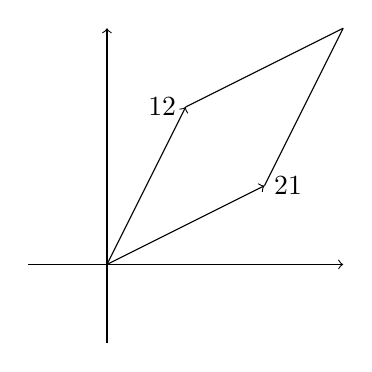
\begin{tikzpicture}[scale=1]
	\draw[->,left] (0,0) node{} -- (1,2) node{$\vv{1}{2}$};
	\draw[->, right] (0,0) node{} -- (2,1) node{$\vv{2}{1}$};
	\draw[] (1,2) node{} -- (3,3);
	\draw[] (2,1) node{} -- (3,3);
	%\draw[->, right] (0,0) node{} -- (2,-1) node{$\V{v}_3$};
	\draw[->] (-1,0) {} -- (3,0) {};
	\draw[->] (0,-1) {} -- (0,3) {};
	\end{tikzpicture}
\end{center}
\end{punkt}


\end{losning}


\begin{oppgave}
La $T$ være tetraederet i $\mathbb{R}^3$ med $(8,8,4)$, $(16,0,0)$, $(1,1,9)$ og~$(8,11,-4)$ som hjørner. Regn ut volumet av $T$.
\end{oppgave}

\begin{losning}
430

\noindent
Hint: Velg et referansepunkt og se på differansen fra de andre vektorene. Du har nå tre vektorer i $\mathbb{R}^3$ som definerer $T$. Observer at $T$ er halvparten av volumet til parallellepipedet definert av vektorene. 
\end{losning}


\begin{oppgave}
La $A$ være matrisen \[
\begin{bmatrix}
\;a & b & 0 & 0\;\\
\;c & 0 & 0 & 0\;\\
\;0 & 0 & 0 & x\;\\
\;0 & 0 & y & z\;
\end{bmatrix}.
\]
\begin{punkt}
Hva er determinanten til $A$ uttrykt ved $a, b, c$ og $x, y, z$?
\end{punkt}

\begin{punkt}
For hvilke verdier av  $a, b, c$ og $x, y, z$ er $A$ inverterbar?
\end{punkt}
\end{oppgave}


\begin{losning}

\begin{punkt}
$bcxy$
\end{punkt}

\begin{punkt}
Vi må ha at $b$, $c$, $x$ og~$y$ alle ikke er lik null.
\end{punkt}

\end{losning}

\begin{oppgave}

Avgjør om følgende påstander er sanne eller ikke. Gi et bevis eller moteksempel i hvert tilfelle.

\begin{punkt}
La $A$ og $B$ være $n\times n$-matriser. Hvis $AB$ er invertibel, så er både $A$ og $B$ invertible.
\end{punkt}

\begin{punkt}
Anta at $A$ er en inverterbar matrise. Da har vi at $$\text{det}(A^{-1})=\frac{1}{\text{det}(A)}.$$
\end{punkt}

\begin{punkt}
Determinanten er definert for alle $m\times n$-matriser.
\end{punkt}

\end{oppgave}

\begin{losning}

\begin{punkt}
Sant.

\noindent
Hint: En matrise er inverterbar hvis og bare hvis determinanten ikke er lik null. Vi vet også at $\text{det}(AB)=\text{det}(A)\text{det}(B)$. Vi har antatt at $\text{det}(AB)\neq 0$. Kan du fullføre beviset?
\end{punkt}

\begin{punkt}
Sant.

\noindent
Hint: $AA^{-1}=I$ og $\text{det}(AB)=\text{det}(A)\text{det}(B)$.
\end{punkt}

\begin{punkt}
Feil; determinanten er kun definert dersom $m=n$.
\end{punkt}

\end{losning}



